
\chapter{Decompositions}

\section{Higher-order singular value decomposition}
Say we have an order $n$ tensor $A$.
We ``unfold'' $A$ along each dimension.
This means pulling the edge $i$ to the left, and flattening the rest to the right.
Then we compute the SVD, $USV$.
Here $U$ is a square matrix, which we keep.
We multiply the $i$th edge of $A$ by $U^T$ (which is also the inverse of $U$).
The result is a ``core'' tensor as well as a sequence of $U$ tensors.
If we want a more compact SVD, we can make each $U$ low rank, like normal SVD.
There is also the ``Interlacing computation`` where we multiply the $U^T$s onto $A$ as we go along.

For order $3$ tensors, this method is called a ``Tucker decomposition''.

% This paper has some reasonably good explanations of improved methods, such as HOOI:
% https://www-users.cse.umn.edu/~saad/PDF/umsi-2006-132.pdf
If the ``core matrix'' is diagonal, this is called tensor rank decomposition.
If we were good at that, we could use it to factor $I^{\otimes 3}$ to get better matrix multiplication algorithms.
Unfortunately tensor rank decomposition is NP hard.

I guess HOSVD gives a rank decomposition if we diagonalize the core tensor.
It just won't be an efficient one.
%What about a method where we first compute a (lower rank) HOSVD, then 

\section{Rank Decomposition}

\subsection{Border Rank}
The border rank of a tensor is the smallest rank of a tensor that is close to it.
TODO: Example where the border rank is much smaller than the rank.

\section{Fast Matrix Multiplication}

Strassen defines 3 tensors of shape $7\times 2\times 2$:
\begin{align*}
S_A &= \begin{bmatrix}
\begin{bmatrix}1 & 0\\0 & 1\end{bmatrix}, &
\begin{bmatrix}0 & 0\\1 & 1\end{bmatrix}, &
\begin{bmatrix}1 & 0\\0 & 0\end{bmatrix}, &
\begin{bmatrix}0 & 0\\0 & 1\end{bmatrix}, &
\begin{bmatrix}1 & 1\\0 & 0\end{bmatrix}, &
\begin{bmatrix}-1 & 0\\1 & 0\end{bmatrix}, &
\begin{bmatrix}0 & 1\\0 & -1\end{bmatrix}
\end{bmatrix}
\\
S_B &= \begin{bmatrix}
\begin{bmatrix}1 & 0\\0 & 1\end{bmatrix}, &
\begin{bmatrix}1 & 0\\0 & 0\end{bmatrix}, &
\begin{bmatrix}0 & 1\\0 & -1\end{bmatrix}, &
\begin{bmatrix}-1 & 0\\1 & 0\end{bmatrix}, &
\begin{bmatrix}0 & 0\\0 & 1\end{bmatrix}, &
\begin{bmatrix}1 & 1\\0 & 0\end{bmatrix}, &
\begin{bmatrix}0 & 0\\1 & 1\end{bmatrix}
\end{bmatrix}
\\
W &= \begin{bmatrix}
\begin{bmatrix}1 & 0\\0 & 1\end{bmatrix}, &
\begin{bmatrix}0 & 1\\0 & -1\end{bmatrix}, &
\begin{bmatrix}0 & 0\\1 & 1\end{bmatrix}, &
\begin{bmatrix}1 & 1\\0 & 0\end{bmatrix}, &
\begin{bmatrix}-1 & 0\\1 & 0\end{bmatrix}, &
\begin{bmatrix}0 & 0\\0 & 1\end{bmatrix}, &
\begin{bmatrix}1 & 0\\0 & 0\end{bmatrix}
\end{bmatrix}
\end{align*}
These tensors have the neat property that they factor $I_2\otimes I_2\otimes I_2$:
\[
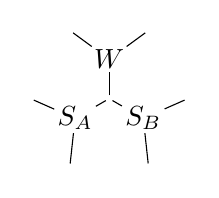
\begin{tikzpicture}[inner sep=1pt, baseline=.0em]
    \node (m) at (0,0) {$\sbullet$};
    \node (W) at (0,.5) {$W$};
    \node (SB) at (-30:.5) {$S_B$};
    \node (SA) at (-150:.5) {$S_A$};
    \node (w1) at (60:1) {};
    \node (w2) at (120:1) {};
    \node (sa1) at (-120:1) {};
    \node (sa2) at (-180:1) {};
    \node (sb1) at (-0:1) {};
    \node (sb2) at (-60:1) {};
    \draw (m) -- (W);
    \draw (m) -- (SA);
    \draw (m) -- (SB);
    \draw (W) -- (w1) {};
    \draw (W) -- (w2) {};
    \draw (SB) -- (sb1) {};
    \draw (SB) -- (sb2) {};
    \draw (SA) -- (sa1) {};
    \draw (SA) -- (sa2) {};
\end{tikzpicture}
=
\begin{tikzpicture}[inner sep=1pt, baseline=.0em]
    \node (m) at (0,0) {};
    \node (W) at (0,.5) {};
    \node (SB) at (-30:.5) {};
    \node (SA) at (-150:.5) {};
    \node (w1) at (60:1) {};
    \node (w2) at (120:1) {};
    \node (sa1) at (-120:1) {};
    \node (sa2) at (-180:1) {};
    \node (sb1) at (-0:1) {};
    \node (sb2) at (-60:1) {};
    \draw (sa2) .. controls (SA) and (W) .. (w2);
    \draw (sa1) .. controls (SA) and (SB) .. (sb2);
    \draw (sb1) .. controls (SB) and (W) .. (w1);
\end{tikzpicture}
.
\]
% TODO: This actually looks like one of the weird plots Penrose makes. Just without the `symmetrization'. Could it be relevant?
%We say that the tensor $I_2\otimes I_2\otimes I_2$ has rank 7, because it can be written as a sum of 7 simple tensors.
%
To multiply two matrices, $A$ and $B$, faster than the normal $n^3$ time,
we reshape them as block matrices, shape $(2,\frac n 2,2,\frac n 2)$ and use Strassen's tensor:
%This means that if we have two $n\times n$ matrices, $A$ and $B$, and we write them as block matrices, shape $2\times \frac n2\times 2\times \frac n2$, we get
\[
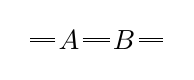
\begin{tikzpicture}[inner sep=1pt, baseline=.0em]
    \node (A) at (-.35, 0) {$A$};
    \node (B) at (.35, 0) {$B$};
    \draw[double] (B) -- ++(.5, 0) {};
    \draw[double] (A) -- ++(-.5, 0) {};
    \draw[double] (A) -- (B) {};
\end{tikzpicture}
=
\begin{tikzpicture}[inner sep=1pt, baseline=-1em]
    \node (m) at (0,0) {};
    \node (W) at (0,.4) {};
    \node (SB) at (-30:.5) {};
    \node (SA) at (-150:.5) {};
    \node (w1) at (.8, 0) {};
    \node (w2) at (-.8, 0) {};
    \node[below=.6em of SA] (A) {$A$};
    \node[below=.6em of SB] (B) {$B$};
    \draw (A) .. controls (-.75,-.5) and (0, 0) .. (w2);
    \draw (A) edge[out=50, in=130] (B);
    \draw (B) .. controls (.75, -.5) and (0, 0) .. (w1);
    \draw (B) -- ++(.5, 0) {};
    \draw (A) -- ++(-.5, 0) {};
    \draw (A) -- (B) {};
\end{tikzpicture}
=
\begin{tikzpicture}[inner sep=1pt, baseline=.0em]
    \node (m) at (0,0) {$\sbullet$};
    \node (W) at (0,.4) {$W$};
    \node (SB) at (-30:.5) {$S_B$};
    \node (SA) at (-150:.5) {$S_A$};
    \node (w1) at (60:1) {};
    \node (w2) at (120:1) {};
    \node (sa1) at (-120:1) {};
    \node (sa2) at (-180:1) {};
    \node (sb1) at (-0:1) {};
    \node (sb2) at (-60:1) {};
    \node[below=.6em of SA] (A) {$A$};
    \node[below=.6em of SB] (B) {$B$};
    \draw (m) -- (W);
    \draw (m) -- (SA);
    \draw (m) -- (SB);
    \draw (W) -- ++(1, 0) {};
    \draw (W) -- ++(-1, 0) {};
    \draw (SB) edge[bend left] (B) {};
    \draw (SB) edge[bend right] (B) {};
    \draw (SA) edge[bend left] (A) {};
    \draw (SA) edge[bend right] (A) {};
    \draw (B) -- ++(.5, 0) {};
    \draw (A) -- ++(-.5, 0) {};
    \draw (A) -- (B) {};
\end{tikzpicture}
.
\]
Contracting the edges in the right order, uses only $7/8 n^3 + O(n^2)$ operations.

If we instead reshape to $(2,2,\dots,2)$,
\[
AB = 
   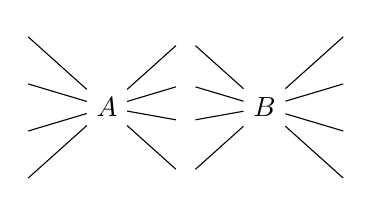
\begin{tikzpicture}[baseline=-1em, y=1.7em]
      \node (P1) at (0,-.5) {$A$};
      \node (A) at (1,1) {};
      \node (P2) at (2,-.5) {$B$};
      \node (B) at (1,0) {};
      \node (C) at (1,-.8) {};
      \node (D) at (1,-2) {};
      \draw (-1,1) -- (P1) -- (A) -- (P2) -- (3, 1);
      \draw (-1,0) -- (P1) -- (B) -- (P2) -- (3, 0);
      \draw (-1,-1) -- (P1) -- (C) -- (P2) -- (3, -1);
      \draw (-1,-2) -- (P1) -- (D) -- (P2) -- (3, -2);
   \end{tikzpicture}
   \,,
\]
and using Strassen's tensor along each axis reduces the work by $(7/8)^{\log_2(n)}$, giving us matrix multiplication in time $n^{3 + \log_2(7/8)} = n^{2.80735}$.


\newpage

Contracting the double edges, $S_A - A$ and $S_B - B$, is both $O(n^2)$ time.

It remains to verify that this is actually faster than the naive matrix multiplication:
Contracting $S_A - A$ takes $7\cdot 2^2 (n/2)^2$ operations, and likewise $S_B - B$.
Next we contract $S_AA - S_BB$ which takes $7(n/2)^3$ time.
And finally we contract the edge with $W$ which takes $2^2 \cdot 7 (n/2)^2$.
The important term is the cubic $7/8 n^3$, which if instead done recursively, leads to the classical $O(n^{\log_2 7})$ algorithm.

FIXME: What ``edge with $W$''? I think we have to/want to contract the hyperedge with $W$ immediately?

\subsubsection{Other}

If we instead wrote $A$ and $B$ using $(n,m)$ and $(m,p)$ shaped blocks, we could factor $I_n\otimes I_m\otimes I_p$ and get a matrix multiplication algorithm using the same approach as the Strassen $(2,2,2)$ tensors above.
Lots of papers have investigated this problem, which has led to the best algorithms by Josh Alman and others.
For example, Deep Mind found a rank 47 factorization of $I_3\otimes I_4\otimes I_5$.

Maybe a more interesting example is the $(4,4,4)$ tensor, for which they find a rank 47 factorization.
This an easy way to create a rank 49 is to take Strassen and double it.
Would this be a nice thing to show? Maybe too messy?
Well, actually their rank 47 construction only works in the ``modular'' case. Then $(3,4,5)$ is general.


